
\section{La corteza cerebral}
La corteza cerebral de los mamíferos es una estructura formada por una gran cantidad de células
nerviosas ($10^{10}$), que en conjunto describen una fina capa de sustancia gris que reviste los hemisferios
cerebrales. Al constituir la porción externa del encéfalo, tempranamente se ha podido describir su
complicada organización macroscópica, en giros, surcos y fisuras, que en el humano muestra un
inconfundible arreglo altamente girificado. Esta organización es el resultado evolutivo de un proceso
que se sugiere comenzó hace 150 millones de años, en la transición del cerebro reptiliano al de los
mamíferos \cite{Valverde2002}.


La corteza cerebral ha sido estudiada desde hace varios siglos, especialmente después de 1776, cuando
Francesco Gennari descubriera la existencia variaciones en la estructura de la corteza cerebral humana,
reportando la existencia de una banda de fibras de sustancia blanca dentro de la corteza, más notorias
en el polo occipital (nombrada banda de Genari, característica de la corteza visual primaria). Estos
datos evidencian uno de los hitos en el estudio de la corteza cerebral: el concepto la no-homogeneidad.
Esta idea guió numerosas investigaciones, sin embargo, se considera que el estudio sistemático de la
estructura de la corteza comenzó con Meynert y Betz en 1867. Ellos estudiaron detalladamente las células que conforman la corteza y concluyeron que, a lo largo de todo el encéfalo, la corteza cerebral presenta un arreglo de 5 capas horizontales, proponiendo dos divisiones principales en la estructura cortical (que corresponderían a lo que Brodmann y Vogt denominaron isocorteza y alocorteza) \cite{fulton_1949}. Aunque desde 1878, Bevan Lewis describió por primera vez la actual estratificación hexalaminar de la isocorteza (Figura \ref{fig:grosor_1}), el concepto de la no-homogeneidad en la arquitectura de la corteza cerebral se consolidó hasta 1909, con los trabajos de Korbinian Brodmann y Cécile y Oskar Vogt. Brodmann y los Vogt parcelaron la corteza cerebral basándose en las variaciones citológicas y en la distribución de fibras conectivas en cada capa, describiendo más de 50 regiones distintas (Figura \ref{fig:grosor_brodmann}). Así mismo, clasificaron la corteza cerebral en dos tipos: isocorteza también llamada neocorteza (distribuida en 6 capas) y alocorteza (3 laminar), a su vez dividida en arquicorteza (hipocampo y giro dentado) y paleocorteza (corteza olfativa)\cite{Valverde2002,brodal_1981}.


\begin{figure}[htb]
\begin{figg}
   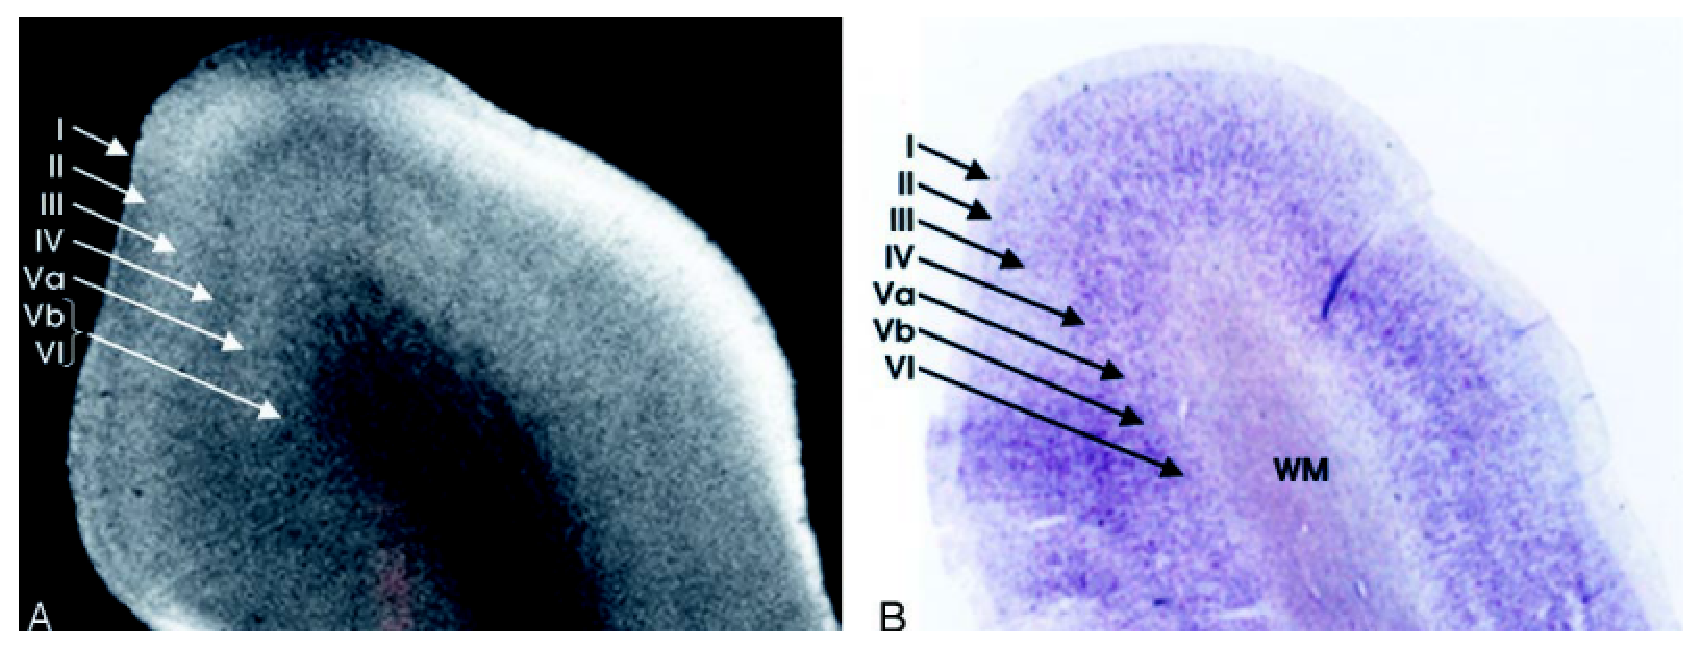
\includegraphics[width=0.7\textwidth]{grosor_1}
   \caption{Imagen por resonancia magnética microscópica de tejido cortical humano, obtenida con 9.4 teslas. Los números romanos indican las capas de la corteza cerebral, las flechas blancas señalan el sitio aproximado de cada capa. Se aprecian tonos oscuros, grises y claros formando bandas dentro de la corteza; en la parte central la elipse oscura corresponde a la sustancia blanca. Las bandas más oscuras como la señalada como IV, presenta plexos horizontales de fibras mielinizadas por lo que pierde intensidad. B. Fotografía de una preparación con Nissl en corteza humana ( giro del polo frontal), corroborando la parcelación laminar. Los números romanos indican la capa y las flechas señalan su sitio aproximado de ubicación. WM: white matter. Modificada de \cite{Fatterpekar2002}. }
 \label{fig:grosor_1}
 \end{figg}
\end{figure}



\begin{figure}[htb]
\begin{figg}
   \includegraphics[width=0.7\textwidth]{grosor_brodmann}
   \caption{Mapa citoarquitectónico de Brodmann.}
 \label{fig:grosor_brodmann}
 \end{figg}
\end{figure}


El estudio de la corteza tuvo un gran avance con en el trabajo de Santiago Ramón y Cajal, quien (utilizando el método de histología desarrollado por Camilo Golgi), logró una descripción muy completa
de la organización intrínseca de la corteza cerebral, describiendo detalladamente la estructura completa
de las células nerviosas (no sólo la distribución de sus somas), con sus proyecciones axonales, y
dendríticas (Tabla \ref{tab:capas_corticales}). De esta manera, se pudo inferir un poco más acerca de la conectividad funcional cortical, estudiando las aferencias y eferencias, así como su distribución en la célula \cite{brodal_1981,fulton_1949}. El estudio de la organización, en láminas horizontales, no sólo brindó información de los diferentes estratos que conforman a la corteza, sino que permitió detectar que las diferentes capas se expanden o desaparecen en determinados sitios corticales. Estos cambios en la citoarquitectura de las capas corticales, son importantes consideraciones, pues aunque que el grosor de la corteza sea mayor o menor en algunas áreas, no debemos perder de vista que eso no significa que todas sus capas se modifiquen en igual proporción.


\begin{table}[]
\centering
\caption{Clasificación  y distribución de las VI capas de la neocorteza cerebral.}
\label{tab:capas_corticales}
\begin{tabular}{p{0.3\textwidth} p{0.7\textwidth}}
\toprule
Capa                          & Descripción                                                                                                                                                                                                                                            \\ \midrule
I. Capa molecular o plexiforme externa & Células horizontales de Cajal, pequeñas células de axón corto, terminaciones de las células piramidales de capas inferiores. Escasas células pero numerosas conexiones horizontales.                                                                            \\
II. Granular externa                   & Células pequeñas tipo piramidal, granular y estrelladas, además de las dendritas basilares y colaterales de las pirámides pequeñas.                                                                                                                             \\
III. Piramidal externa                 & Celulas piramidales medianas y grandes.                                                                                                                                                                                                                         \\
IV. Granular interna                   & Células estrelladas pequeñas con dendritas distribuidas a lo largo de la capa, granulares y piramidales estrelladas con colaterales horizontales axónicas y dendríticas. Suele ser la más delgada excepto en las cortezas sensoriales. Capa altamente fibrilar. \\
V. Piramidal interna o ganglionar      & Piramidales medianas y grandes (p. ej. piramidales gigantes de Betz), con colaterales dentro de la misma capa, constituye la principal eferencia subcortical. La subcapa Vb contiene plexos horizontales de fibras mielinizadas.                                  \\
VI. Multiforme                         & Células de forma irregular, fusiformes o polimorfas. El estrato más basal contacta con  la sustancia blanca (Vib).                                                                                                                                              \\ \bottomrule
\end{tabular}
\end{table}

Con estos datos queda claro que la corteza cerebral constituye una de las estructuras más complejas del
sistema nervioso, que ha sido estudiada durante siglos, desde diferentes aproximaciones conceptuales
y metodológicas, pero todas en busca de datos que revelen su papel en el procesamiento de información
y en general, la relación entre la estructura y la función cortical.



\section{Grosor cortical}

Aunque hemos descrito brevemente que la corteza cerebral es una estructura heterogénea (formada por
diversos tipos celulares con intrincados patrones de conectividad), vista macroscópicamente forma una capa relativamente uniforme y notoriamente distinta de la capa interna inmediata, es decir, de la
sustancia blanca. La sustancia blanca está formada por numerosos tractos axonales que comunican, en
ambas direcciones, a la corteza cerebral con estructuras y núcleos subcorticales \cite{brodal_1981}. Esta
organización de la sustancia gris y la sustancia blanca, permite una división ordenada de los cuerpos
celulares corticales y, por ende, una disposición radial conjunta de todas sus proyecciones y aferencias.
Este arreglo celular permite que el espacio entre cada cuerpo celular sea considerablemente menor que
si estuviesen mezclados los somas neuronales con todas las fibras \cite{Shipp_2007}. Sin embargo,
metodológicamente hablando, lo que permite es una estimación refinada e independiente de ambos
sustratos. 

El grosor cortical, como definición operacional, corresponde al espacio contenido entre la sustancia
blanca y la superficie pial \cite{Lerch_Evans_2005}. Antiguamente, el grosor cortical del cerebro humano sólo
podía ser estudiado \emph{post mortem} (habitualmente secundario a patología o trauma), por lo que
difícilmente se podía acceder a información de la fisiología normal. Asimismo, cualquier tejido
biológico sometido a un proceso de preservación, sin importar el método de fijación, presentará, en
mayor o menor grado alteraciones en la citoarquitectura del tejido (p. ej. paraformaldehído, nicromato
de potasio y tetraóxido de osmio). Aunado a lo anterior, cabe mencionar que el estudio del grosor
cortical por método de disección, es una tarea harto compleja, no sólo por la precisión y entrenamiento
quirúrgico que demanda, sino por la irregularidad del tejido, con giros e invaginaciones que pueden ser
tan profundas que en algunas partes resulta muy inaccesible su estudio (p. ej. la corteza insular)
Entre las bondades de la IRM estimando el grosor cortical están: una buena resolución anatómica, su naturaleza no invasiva y, sobre todo, posibilita el diagnóstico temprano de estados patológicos \cite{Dickerson2001,Kaye1997,Rosas2002}. Actualmente, la IRM ha permitido visualizar y
estimar el grosor de la corteza humana in vivo y a lo largo de la vida \cite{Salat1999a,Sowell2003}.
Los datos actuales muestran que en promedio la corteza cerebral humana presenta un grosor entre 2 y 5
mm, y que este varia dependiendo de la región cortical que se observe (p. ej. mayor grosor en cortezas
sensoriales) \cite{Fischl_Dale_2000,Shipp_2007}. La IRM posibilitó el estudio sistemático
del grosor cortical durante el envejecimiento natural \cite{Jack_1997,Sowell2003}, aunque los cambios
más impresionantes, en grosor y volumen, parecen ocurrir durante el desarrollo temprano,
especialmente durante el primer año de vida (Figura \ref{fig:grosor_desarrollo}) \cite{Nie2012}.


\begin{figure}[htb]
\begin{figg}
   
\includegraphics[width=\textwidth]{grosor_desarrollo}
   \caption{Imágenes por resonancia magnética, obtenidas con contraste tipo \Tone. Vista axial de 6 cerebros de neonatos en diferentes puntos temporales: 2 semanas, 3 , 6 , 9 y 12 meses (de izquierda a derecha). Cambios en el volumen, grosor cortical y patrones de girificación del encéfalo humano a lo largo del desarrollo del primer año de vida. Modificada de \cite{Nie2012}.
}
 \label{fig:grosor_desarrollo}
 \end{figg}
\end{figure}


Un dato de relevancia metodológica que vale la pena mencionar, refiere a las comparaciones hechas
entre los datos del grosor cortical de diferentes regiones corticales (mediales, laterales, inferiores, etc),
obtenidos por IRM y las estimaciones realizadas con técnicas histológicas \textit{pos mortem}. Estas
comparaciones han mostrado correlaciones en las estimaciones del grosor cortical entre las dos
técnicas, sin olvidar que en ambas se presentan limitantes en la estimación (p.ej. daños en la
microestructura en el tratamiento de los tejidos para histología o los errores de estimación en RM). Este
dato demuestra la confiabilidad de la IRM como técnica, considerando su baja resolución espacial para
ciertos detalles neuroanatómicos  \cite{Fatterpekar2002,Fischl1999_cortical}.

\section{Consideraciones en la estimación del grosor cortical} 
Esta sección y la siguiente describen, de manera general, las técnicas utilizadas en IRM para la
adquisición y el análisis de imágenes, con la finalidad última de explotar características que faciliten la
segmentación de la corteza, es decir, de distinguirla de todo aquello que no sea corteza (meninges,
líquido cefalorraquídeo, sustancia blanca). La variación en el contraste (diferencias de intensidad) entre
la sustancia gris y la sustancia blanca, es una característica determinante en este proceso.
Si bien es cierto que muchos tipos de análisis dentro de la IRM son automatizados, el procesamiento
para calcular del grosor cortical es largo y requiere de revisión y posible corrección manual, en varios
puntos del proceso. Independientemente del análisis que se escoja para estimar el grosor cortical,
existen dificultades comunes, que van en relación a su diseño. Al ser una superficie curva, la corteza
cerebral presenta pliegues irregulares con giros y surcos (algunos muy profundos y angostos), que
muchas veces resultan en segmentos donde el espacio entre dos puntos distintos de la corteza es
mínimo, lo que complica la elección del ángulo de medición (Figura \ref{fig:grosor_surcos}).

\begin{figure}[htb]
\begin{figg}
   
\includegraphics[width=0.7\textwidth]{grosor_surcos}
   \caption{Imagen por resonancia magnética con contraste tipo \Tone, vista coronal del lóbulo temporal. La banda más obscura corresponde a la corteza cerebral, toda la superficie clara es sustancia blanca. El círculo negro señala una región de extremo contacto entre distintas superficies de la corteza.
}
 \label{fig:grosor_surcos}
 \end{figg}
\end{figure}



Para estimar el grosor cortical se suelen utilizar imágenes por RM que, como ya mencionamos,
potencien el contraste entre tejidos y tal es el caso de las secuencias pesadas a \Tone. Las imágenes tipo
\Tone permiten el máximo contraste entre la sustancia blanca y la sustancia gris, para lograrlo se utilizan
parámetros de adquisición específicos en la temporalidad de los pulsos de excitación, en la lectura del
eco y en el tiempo de inversión. Sin embargo, de igual importancia es la resolución que se utiliza en la
adquisición de la imagen, por lo que, lo más común es utilizar adquisiciones en 3 dimensiones. La
tridimensionalidad otorga mayor resolución a la imagen, debido a que se añade un nuevo gradiente en
la codificación de la fase y al mismo tiempo mejora la relación señal-ruido (SNR, por sus siglas en
inglés). En promedio se utiliza una resolución de 1 mm${^3}$, procurando no exceder 1.5 mm${^3}$ en el grosor
del voxel (Tabla \ref{tab:grosor_protocolos}). Este tipo imágenes se obtienen con secuencias eco de gradiente (GE, por sus siglas en inglés) o de Inversión/recuperación (IR, por sus siglas en inglés). La mayoría de los resonadores
comerciales incluyen estos protocolos de manera estándar, como las secuencias 3D MP-RAGE (en
protocolos de resonadores Siemens) o 3D SPGR (en protocolos de resonadores General Electric).

% Please add the following required packages to your document preamble:
% \usepackage{booktabs}
\begin{table}[]
\centering
\caption{Ejemplo de dos protocolos de adquisición de imágenes, útiles para estimar el grosor cortical.}
\label{tab:grosor_protocolos}
\begin{tabular}{@{}lll@{}}
\toprule
Parámetro                     & General Electric & Siemens    \\ \midrule
Nombre                        & 3D SPGR          & 3D MP-RAGE \\
Angulo de desviación (grados) & 25               & 10         \\
TR (ms)                       & 9                & 9.7        \\
TI (ms)                       & 2.1              & 4          \\
TE (ms)                       & 300              & 20         \\
Resolución (mm)               & 1$\times$1$\times$1            & 1$\times$1$\times$1      \\ \bottomrule
\end{tabular}
\end{table}



Finalmente, la última consideración antes de abordar el procedimiento y técnicas para la medición del
grosor cortical con IRM, considera todos los temas antes mencionados. Aunque poco hemos hablado
de la sustancia blanca que subyace a la corteza, excusándonos en su sofisticado arreglo que permite
distinguirla fácilmente de la sustancia gris, cabe mencionar que estas fibras (corticofugas y centrípetas)
tienen un arreglo muy preciso en su trayectoria desde o hacia determinadas capas, formando columnas
que siguen un cierta curvatura que debe considerarse (Figura \ref{fig:grosor_fibrasradiales}).


\begin{figure}[htb]
\begin{figg}
   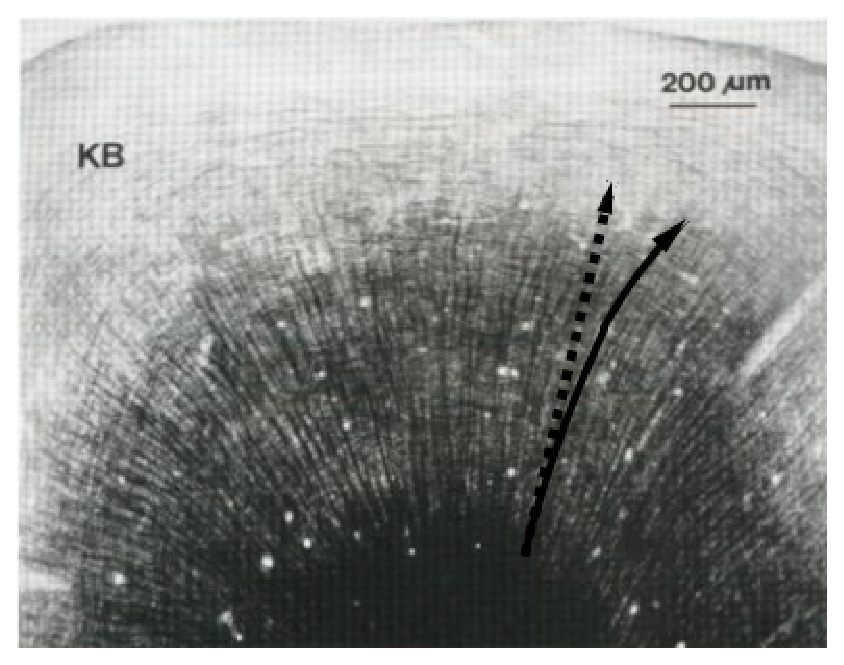
\includegraphics[width=0.7\textwidth]{grosor_fibrasradiales}
   \caption{Fotografía de un corte de corteza cerebral procesado para detectar mielina. Las fibras se distribuyen geométricamente en la corteza. La flecha punteada señala una medición de grosor cortical sin considerar este patrón; la flecha sólida se distribuye considerando la organización fibrosa (Modificada de Lerch J. [falta ref. completa]).
}
 \label{fig:grosor_fibrasradiales}
 \end{figg}
\end{figure}




\section{Análisis del grosor cortical}
Los dos métodos más utilizados para estudiar el grosor cortical, son la morfometría basada en voxeles
(VBM, por sus siglas en inglés) y la morfometría basada en el análisis de superficie (SBM, por sus siglas en inglés). La VBM como parte de los métodos volumétricos, estima las variaciones locales en el volumen de la sustancia gris, para generar mapas tisulares representando la concentración de
sustancia gris, voxel por voxel (Capítulo \ref{chapter_vbm}). Sin embargo, para medir el grosor cortical o el grado de girificación de una corteza, la VBM no es la mejor opción. La SBM posibilita la extracción de más
información como: el espesor cortical, el grado de girificación, el grado de curvatura, la forma del giro
o la profundidad del surco. Por lo anterior, nos enfocaremos en la SBM como método para cuantificar
y estudiar el grosor cortical. 

Lo primero con lo que se debe contar para iniciar el análisis las imágenes estructurales (generalmente
pesadas a \Tone), adquiridas con las características descritas previamente. Estas imágenes, son
consideradas la materia prima, que será sometida a los siguientes procedimientos (Figura \ref{fig:grosor_pasos}):


\begin{description}

 \item [Registro y alineación.] En esta parte del proceso las imágenes estructurales (el primer volumen) se
registran (registro lineal) y alinean con relación a un atlas. Los atlas más usados son el de Talairach y
Tournoux, y el MNI152. Este paso calcula los parámetros de transformación para maximizar la
similitud entre el volumen individual y el volumen promedio de varios sujetos previamente alineados
(atlas), transformando las coordenadas originales de la imagen a las coordenadas de Talairach.

\item [Normalización de la intensidad.] Este es uno de los pasos más importantes en el tratamiento de la
imagen, debido a que resuelve las diferencias en la intensidad de la imagen que se haya producido por
pequeñas inhomogeneidades del campo magnético o de las antenas de radiofrecuencia, generando que
tejidos similares presenten intensidades distintas. Considerando que la estimación y segmentación del
grosor cortical se basa en las diferencias en la intensidad de los tejidos, es importante eliminar diferencias que se deban a artefactos. La normalización se basa en el principio de que en cualquier
rebanada el pico máximo de intensidad será dado por la sustancia blanca. Este valor se usa para fijar en
un valor la media de la intensidad de la sustancia blanca, ésto para cada rebanada. Los voxeles de
sustancia blanca que hayan quedado sin clasificar como sustancia blanca (campo de sesgo), pueden ser
corregidos mediante ``puntos de control'' que incluyen estos nuevos valores de intensidad como
sustancia blanca. Utilizando el algoritmo de partición de Voronoi, se calcula el campo de sesgo en los
voxeles sin etiquetar, de tal forma que en estos puntos se asigna el valor del punto de control más
cercano. Para asignar estos valores, se realiza un suavizado de la imagen, donde se sustituyen los
puntos o voxeles de ``no-control'' por el promedio de intensidad ese mismo voxel y de los 26 voxeles
adyacentes, suavizando los límites entre las regiones hechas por el algoritmo de Voronoi.

\item [Extracción virtual del cerebro.] Este paso utiliza la imagen normalizada para eliminar de la imagen la
piel, el cráneo y las meninges. Para eliminar todo lo mencionado, se emplea un molde generado
mediante deformaciones graduales de una elipsoide, la cual se expande gradualmente, moldeándose,
hasta describir un cerebro promedio. Este molde es superpuesto en la imagen normalizada, y permite la
eliminación de casi todos los voxeles que se localizan fuera del molde del cerebro.

\item [Segmentación.] Este proceso automático conlleva dos pasos, el primero clasifica cada voxel
dependiendo de su intensidad. Posteriormente, se examina y con relación a un mapa probabilístico
(basado en segmentaciones manuales en un atlas) se clasifica en sustancia blanca del hemisferio
derecho o izquierdo, sustancia gris, o algunas estructuras subcorticales. Al obtener información de la
segmentación automática y de las clasificaciones de intensidades se obtiene un valor de la probabilidad
conjunta, que permite catalogar más precisamente la imagen en varios tipos de tejidos. Para el análisis
de la corteza cerebral, lo más importante de este paso es la distinción entre sustancia gris y sustancia
blanca, por ende este paso suele ser referido como segmentación de la sustancia blanca.

\item [Planos de corte.] Una vez segmentada la imagen, se generan representaciones de cada hemisferio
cerebral, utilizando dos planos de corte. El primero es un corte sagital a lo largo del cuerpo calloso, que separa a los dos hemisferios; el segundo, es horizontal y se realiza a nivel del puente. Este último corte
elimina las estructuras subcorticales y genera dos superficies topológicamente cerradas.

\item [Conexión de componentes.] En este paso, se unifica la segmentación realizada para generar una
reconstrucción de toda la materia blanca en cada hemisferio que incorpora todos los elementos aislados
dentro de cada hemisferio, siendo ``rellenados'' y convertidos en voxeles de sustancia blanca. De esta
forma se construyen dos representaciones (para cada hemisferio) de voxeles interconectados.

\item [Deformar, refinar y teselar superficies.] Las dos superficies de sustancia blanca generadas en el paso
anterior, son representadas en un mosaico (teselado) que se construye representando cada cara de un
voxel con dos triángulos, considerando que las caras de los voxeles son necesariamente ortogonales a
alguno de los ejes cardinales, el mosaico resultante tiende a ser irregular. Para corregir la irregularidad
generada, la superficie (en mosaico) es sometida a un proceso de suavizado utilizando un algoritmo de
superficie deformable basado en las variaciones locales de la intensidad en la IRM; algo muy
importante es que la topología no cambia a lo largo de este proceso. Esta superficie deformable (que
ahora es representada por vértices y aristas) constituye el límite inferior de la corteza cerebral. Una vez
que se tiene representada la sustancia blanca en una superficie, ésta habrá de extenderse (a partir de una
esfera), hasta que encuentra los límites (por intensidad) de la sustancia gris con la pía madre. Una vez que
encuentra estos límites, la esfera ya se ha deformado a una superficie que visualmente semeja los giros
y surcos de la imagen original. La distancia entre la superficie de sustancia blanca y la sustancia gris
determina el grosor cortical. La flexibilidad del globo para deformarse en la superficie cortical
dependerá de las características de la malla, como el número de vértices \cite{Dale1999}.
\end{description}


\begin{figure}[htb]
\begin{figg}
   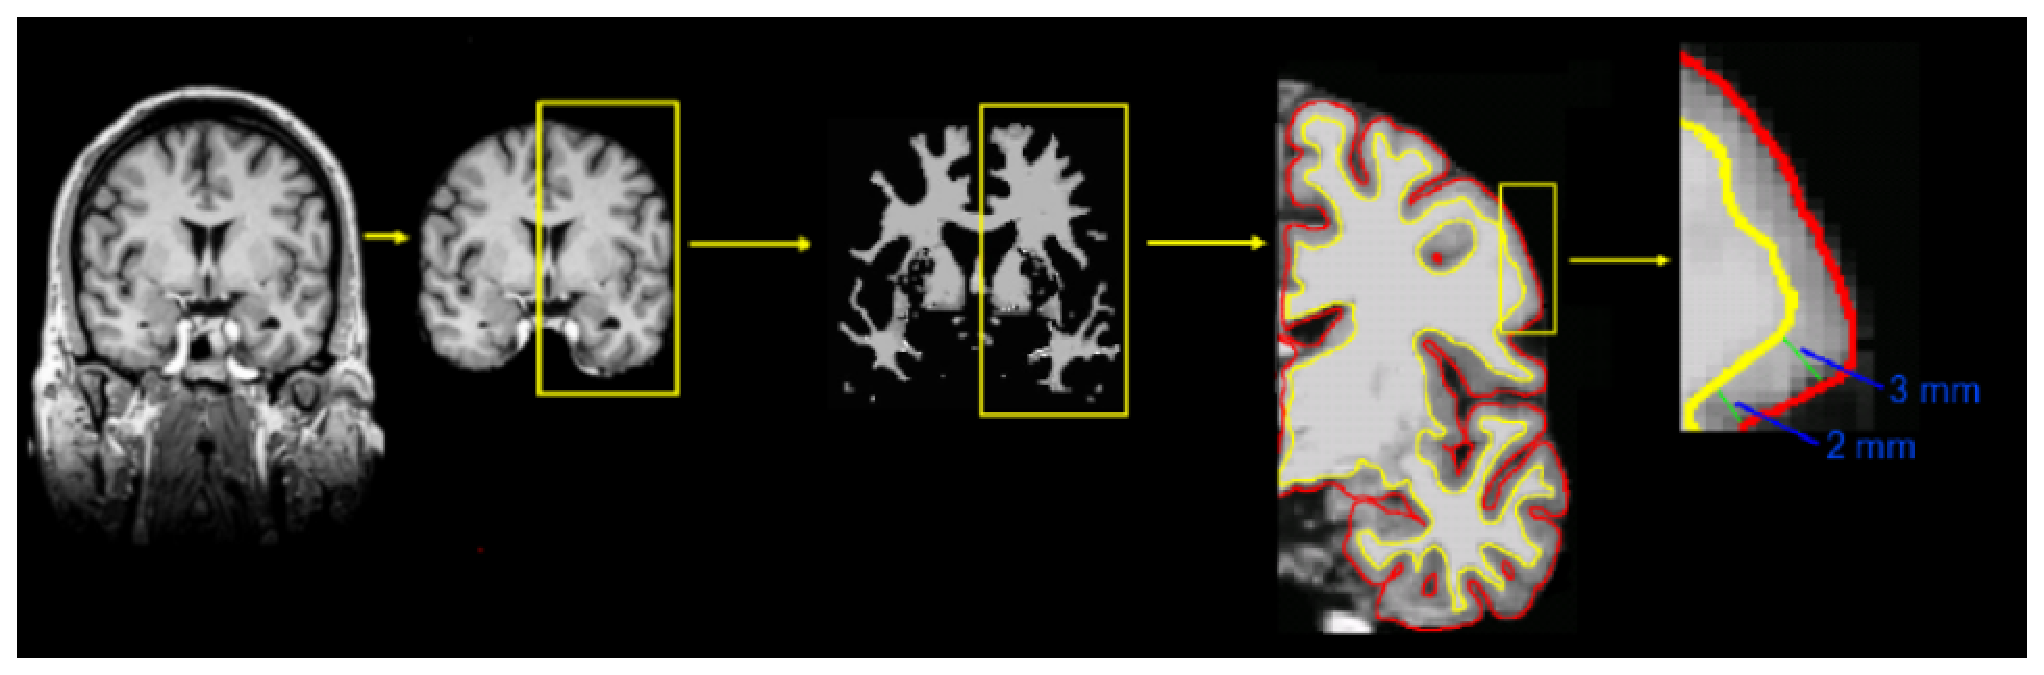
\includegraphics[width=\textwidth]{grosor_pasos}
   \caption{Imágenes por resonancia magnética (contraste \Tone) en vistas coronales. Cada imagen ejemplifica un paso en el procesamiento de para estimar grosor cortical, de izquierda a derecha se observan: la imagen original; la imagen resultante de la extracción de cerebro; la segmentación de la sustancia blanca; amplificación del recuadro amarillo mostrando las dos líneas que segmentan la sustancia blanca (línea amarilla) y la sustancia gris (línea roja); finalmente, amplificación a mayor aumento de un giro cortical con estimaciones promedio de del grosor cortical señalado por las líneas verdes.
}
 \label{fig:grosor_pasos}
 \end{figg}
\end{figure}





De manera general, estos son los pasos necesarios para procesar una imagen y calcular el grosor
cortical, existen diferentes \textit{softwares} para su análisis como \textit{Freesurfer} (MGH, Harvard) o \textit{CIVET} (BIC, Montreal). Sin embargo, aunque la mayoría de los \textit{softwares} emplean alrededor de 40 horas en este análisis (por cada sujeto), existen otros métodos que pueden estimar superficies el proceso en menos de 1 hora, aunque tienen considerables inconveniencias para el análisis entre sujetos (p. ej. no hay correspondencia de vértices). Así mismo cada software utiliza distintos estimadores para el cálculo de las propiedades morfológicas de la corteza, entre ellas el grosor cortical. En la Figura \ref{fig:grosor_mediciongrosor} se muestran cuatro formas distintas de medir el espesor cortical. El método de superficie define el grosor cortical como la distancia Euclidiana entre los puntos correspondientes entre la superficie interior y exterior. Por su parte, el método de puntos más cercanos (b) calcula la distancia más cercana entre un cada punto de una superficie con otro punto de la otra superficie. Los métodos Laplacianos (c) calculan el grosor cortical considerando una curvatura en oposición a las mediciones por línea recta, como la anterior, resultando en un cálculo un poco más preciso que conserva propiedades geométricas similares a las de las columna funcionales de la corteza cerebral. Otros métodos (d) utilizan círculos que se expanden dentro de la delimitación de la corteza cerebral y calculan el espesor contenido dentro de cada círculo como una medida para evitar los efectos de volumen parcial \ref{Lerch_Evans_2005,Thorstensen_measuringcortical}.


\begin{figure}[htb]
\begin{figg}
   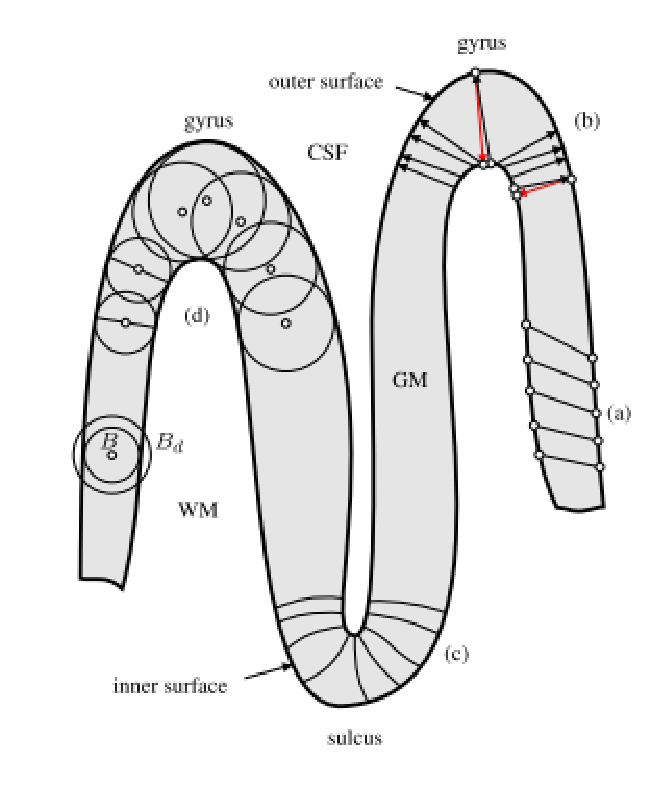
\includegraphics[width=0.7\textwidth]{grosor_mediciongrosor}
   \caption{Esquema de los diferentes métodos para medir el grosor cortical (a-d). La banda azulada representa la corteza cerebral (GM); CSF, líquido cefalorraquídeo; WM, sustancia blanca (Modificado de \ref{Thorstensen_measuringcortical})
}
 \label{fig:grosor_mediciongrosor}
 \end{figg}
\end{figure}



La finalidad de este tipo de análisis, generalmente, es la comparación entre grupos, por lo que la
correspondencia anatómica de los vértices (entre sujetos) cobra suma importancia. De ahí la relevancia
de tomarse el tiempo necesario para un procesamiento adecuado (~ 40 hrs) de la imagen, que posibilite
realizar estadísticas hechas voxel por voxel (comparaciones múltiples), entre sujetos o grupos
experimentales.

A medida que se perfecciona el software para el estudio del grosor cortical, han venido surgiendo nuevas y vistosas formas de representar la corteza y facilitar su análisis cuantitativo o su inspección visual. Entre estas técnicas, una ampliamente utilizada implica la representación esférica de la corteza cerebral, esta superficie puede incluir la distinción con colores entre giros y surcos (p. ej. giros/gris claro y surcos/gris obscuro), que posteriormente puede visualizarse en dos dimensiones y facilitar la visualización de áreas corticales inaccesibles de otra manera (p.ej. surcos profundos) (Figura \ref{fig:grosor_flat}).

\begin{figure}[htb]
\begin{figg}
   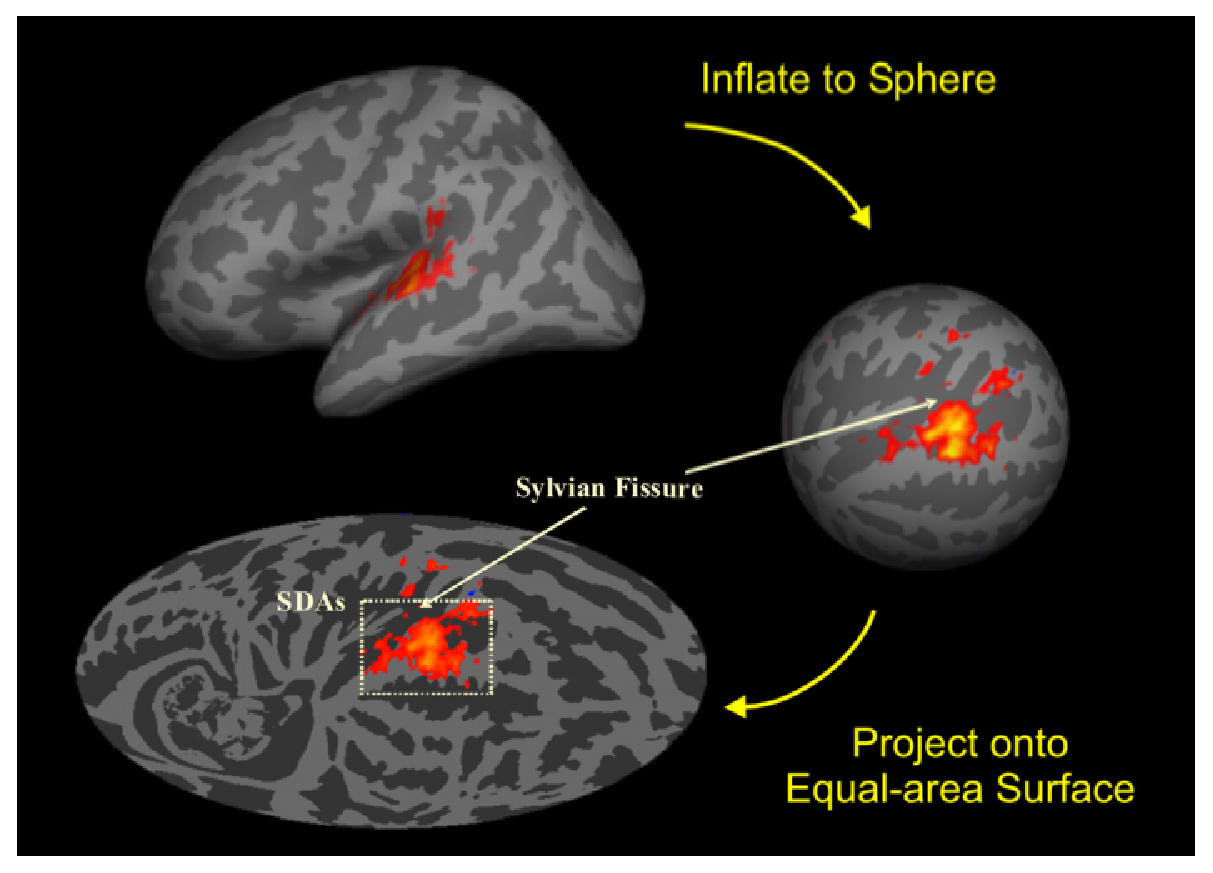
\includegraphics[width=0.7\textwidth]{grosor_flat}
   \caption{Representación de la corteza cerebral en superficies. Transformación de una proyección en 3D conservando la forma del cerebro, a una representación esférica y finalmente a una superficie plana. Los grises claros representan giros y los grises oscuros representan los surcos (Modificada de \cite{Woods_2009}.
}
 \label{fig:grosor_flat}
 \end{figg}
\end{figure}


